\subsubsection{SWITCH} \label{sssec:switch}

Results with sequential switching are shown in Figs. \ref{fig:Hval_Switch} to \ref{fig:MP_Switch}.
The calculated entropy value for floating-point implementation is $\left\langle H_{hist}\right\rangle =0.9722$, this value is slightly higher than the one obtained for the LOG map. 
For fixed-point arithmetic this value is reached in $B=24$, but it stabilizes from $B=28$.
Regarding the ordering patterns the number of MP decreases to $586$, this value is lower than the one obtained for LOG map.
It means the entropy $H_{BP}$ may increase up to $\ln(134)/\ln(720)\simeq 0.74$.
BP and BPW quantifiers reach their maximum of $\left\langle H_{BP}\right\rangle =0.6546$ and $\left\langle H_{BPW}\right\rangle =0.6313$ at $B=16$, but they stabilize from $B=24$.
Complexities are lower than for LOG, $\left\langle C_{BP}\right\rangle =0.4580$ and $\left\langle C_{BPW}\right\rangle =0.4578$, these values are reached for $B \geq 15$ but they stabilize for $B \geq 23$.
Compared with LOG, statistical properties are better with less amount of bits, for $B \geq 24$ this map reaches optimal characteristics in the sense of random source.

Furthermore, we encountered one initial condition in floating-point long double precision with an anomalous behavior
Figs. \ref{fig:Hval_Switch}, \ref{fig:Hbp_Switch} and \ref{fig:Cbp_Switch} show an horizontal blue dashed line that is far from the average value, unlike this is not detected by quantifiers based on $BPW$ procedure in Figs. \ref{fig:Hbpw_Switch} and \ref{fig:Cbpw_Switch}.
Nevertheless comparing both procedures ($BP$ and $BPW$) we were able to detect a falling to fixed point after a long transitory, the BPW procedure discards the constant values (corresponding with a fixed point) and works only over the transitory values.

\begin{figure}[H]
	\centering
	\begin{subfigure}[b]{0.49\textwidth}
		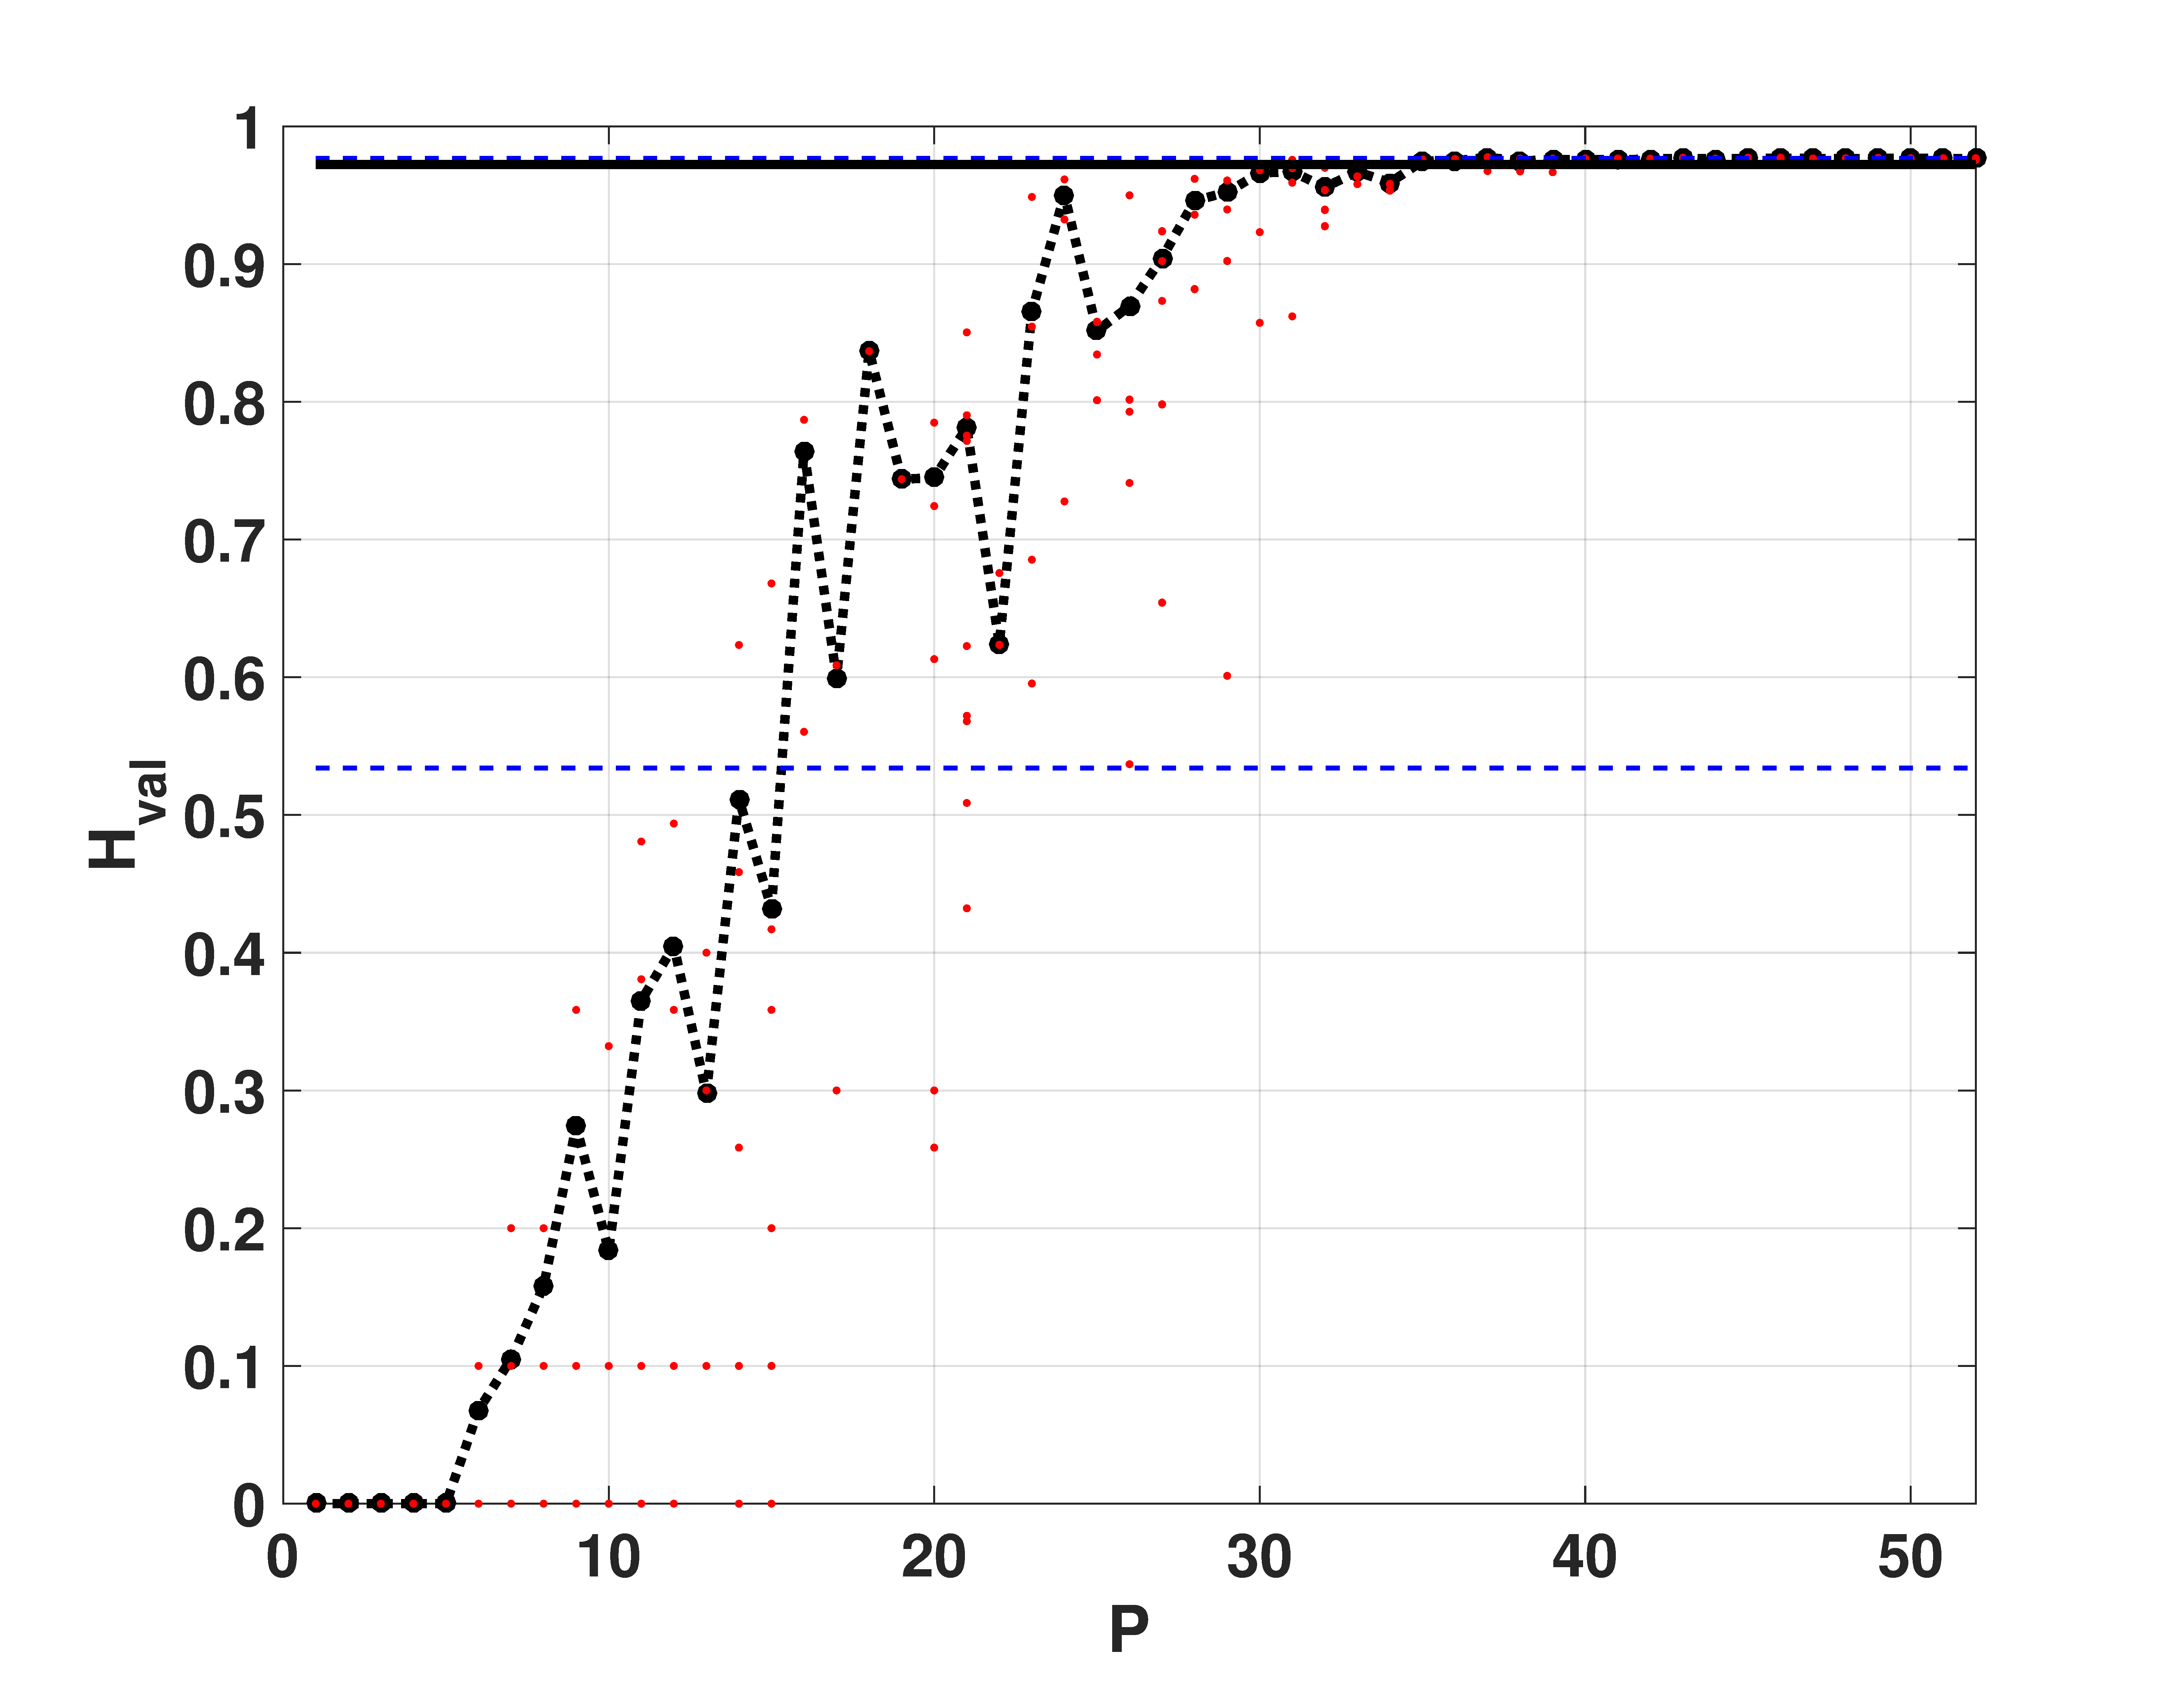
\includegraphics[width=\textwidth]{Hval_Switch}
		\caption{$H_{hist}$ vs. $B$}
		\label{fig:Hval_Switch}
	\end{subfigure}
	\begin{subfigure}[b]{0.49\textwidth}
		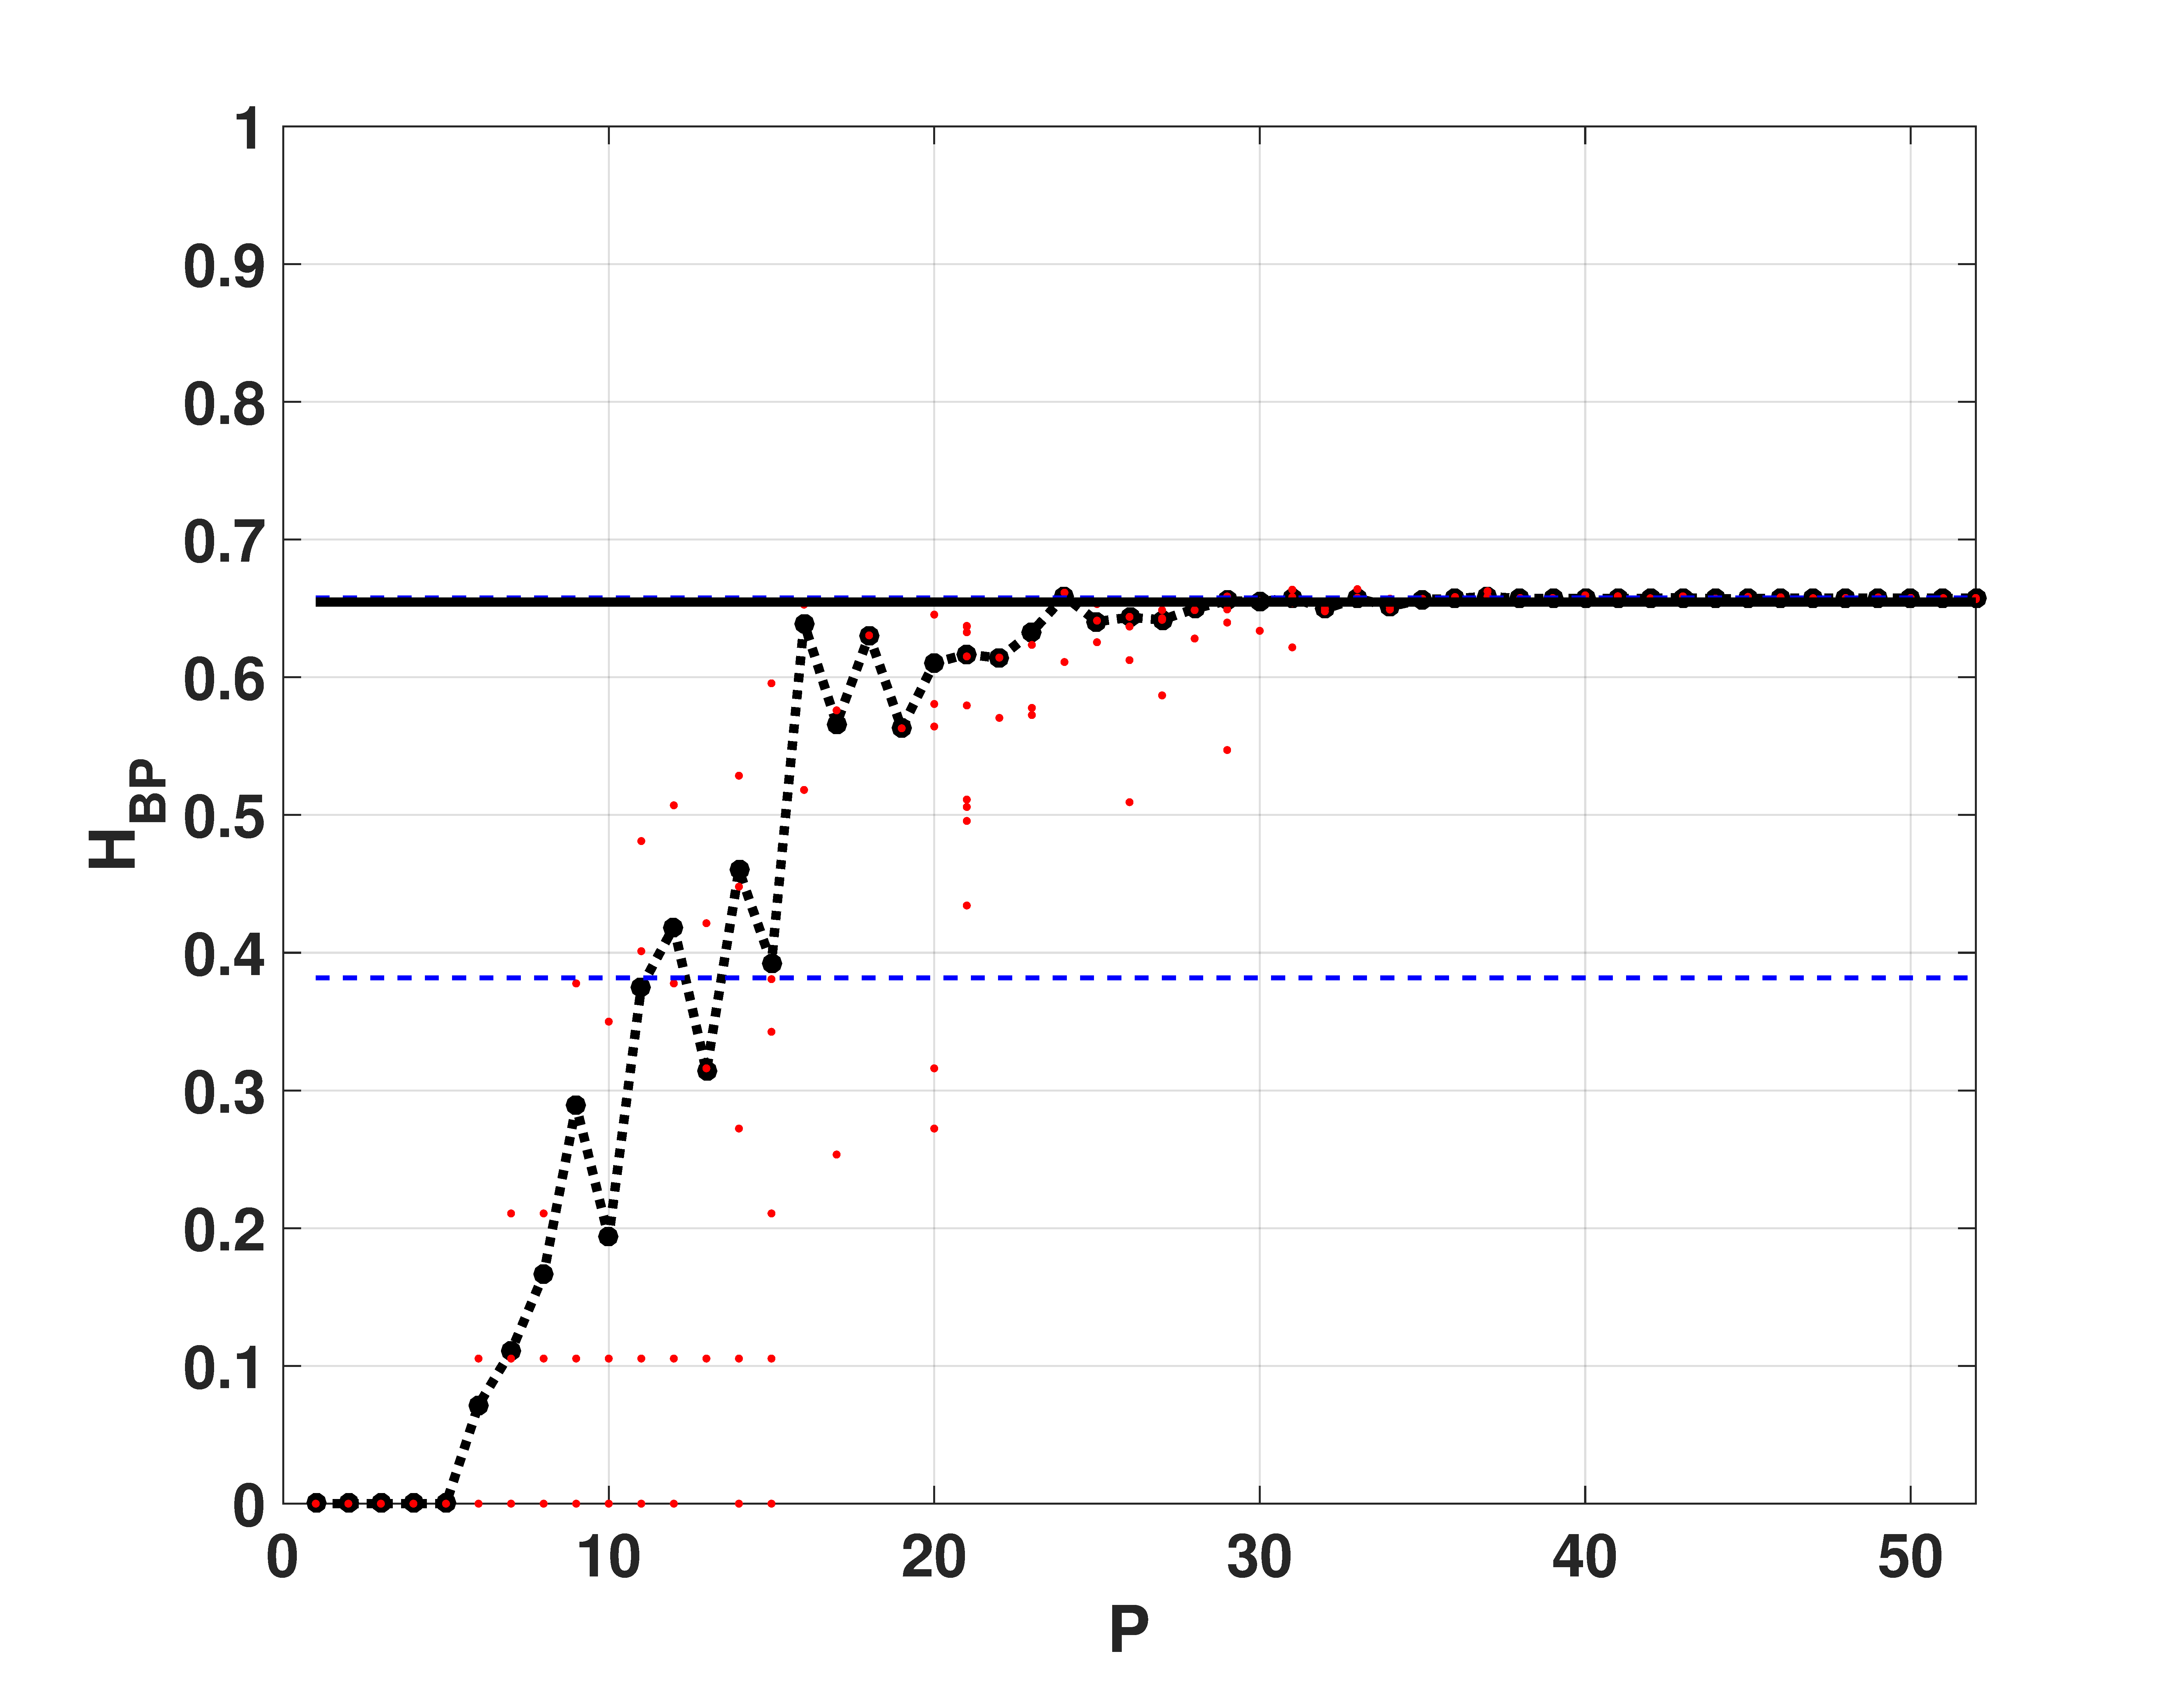
\includegraphics[width=\textwidth]{Hbp_Switch}
		\caption{$H_{BP}$ vs. $B$}
		\label{fig:Hbp_Switch}
	\end{subfigure}
	\begin{subfigure}[b]{0.49\textwidth}
		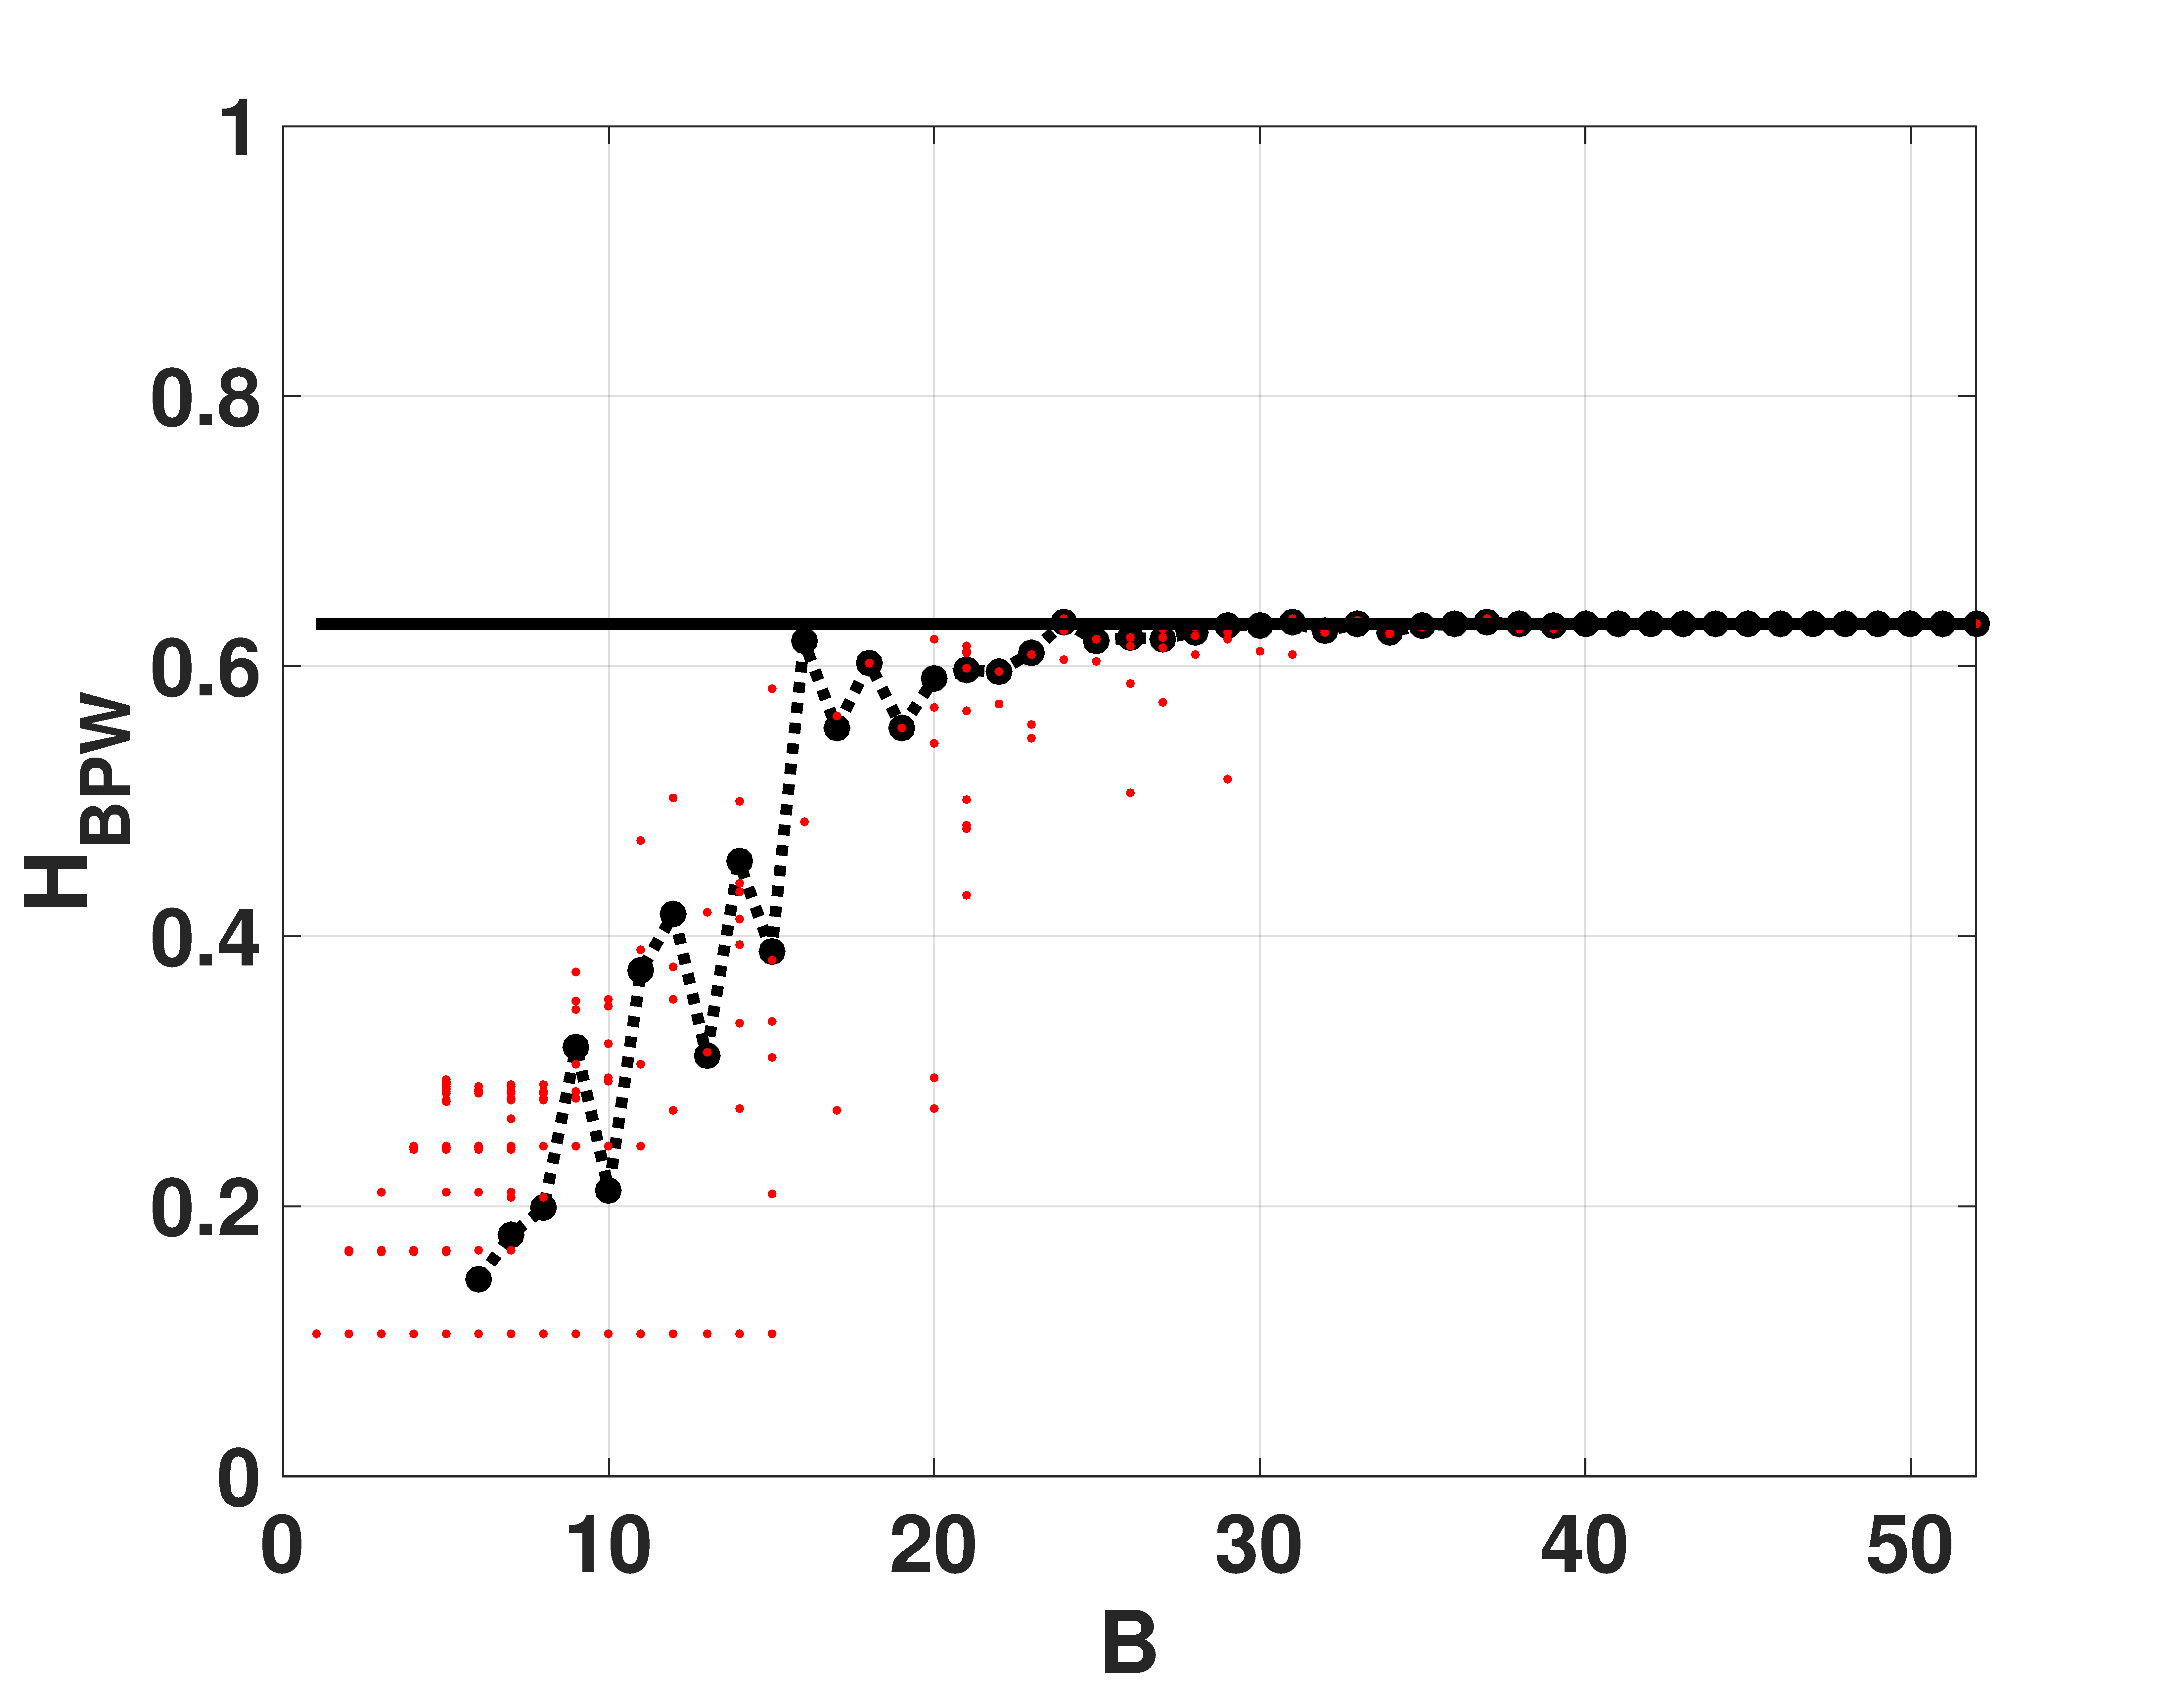
\includegraphics[width=\textwidth]{Hbpw_Switch}
		\caption{$H_{BPW}$ vs. $B$}
		\label{fig:Hbpw_Switch}
	\end{subfigure}
	\begin{subfigure}[b]{0.49\textwidth}
		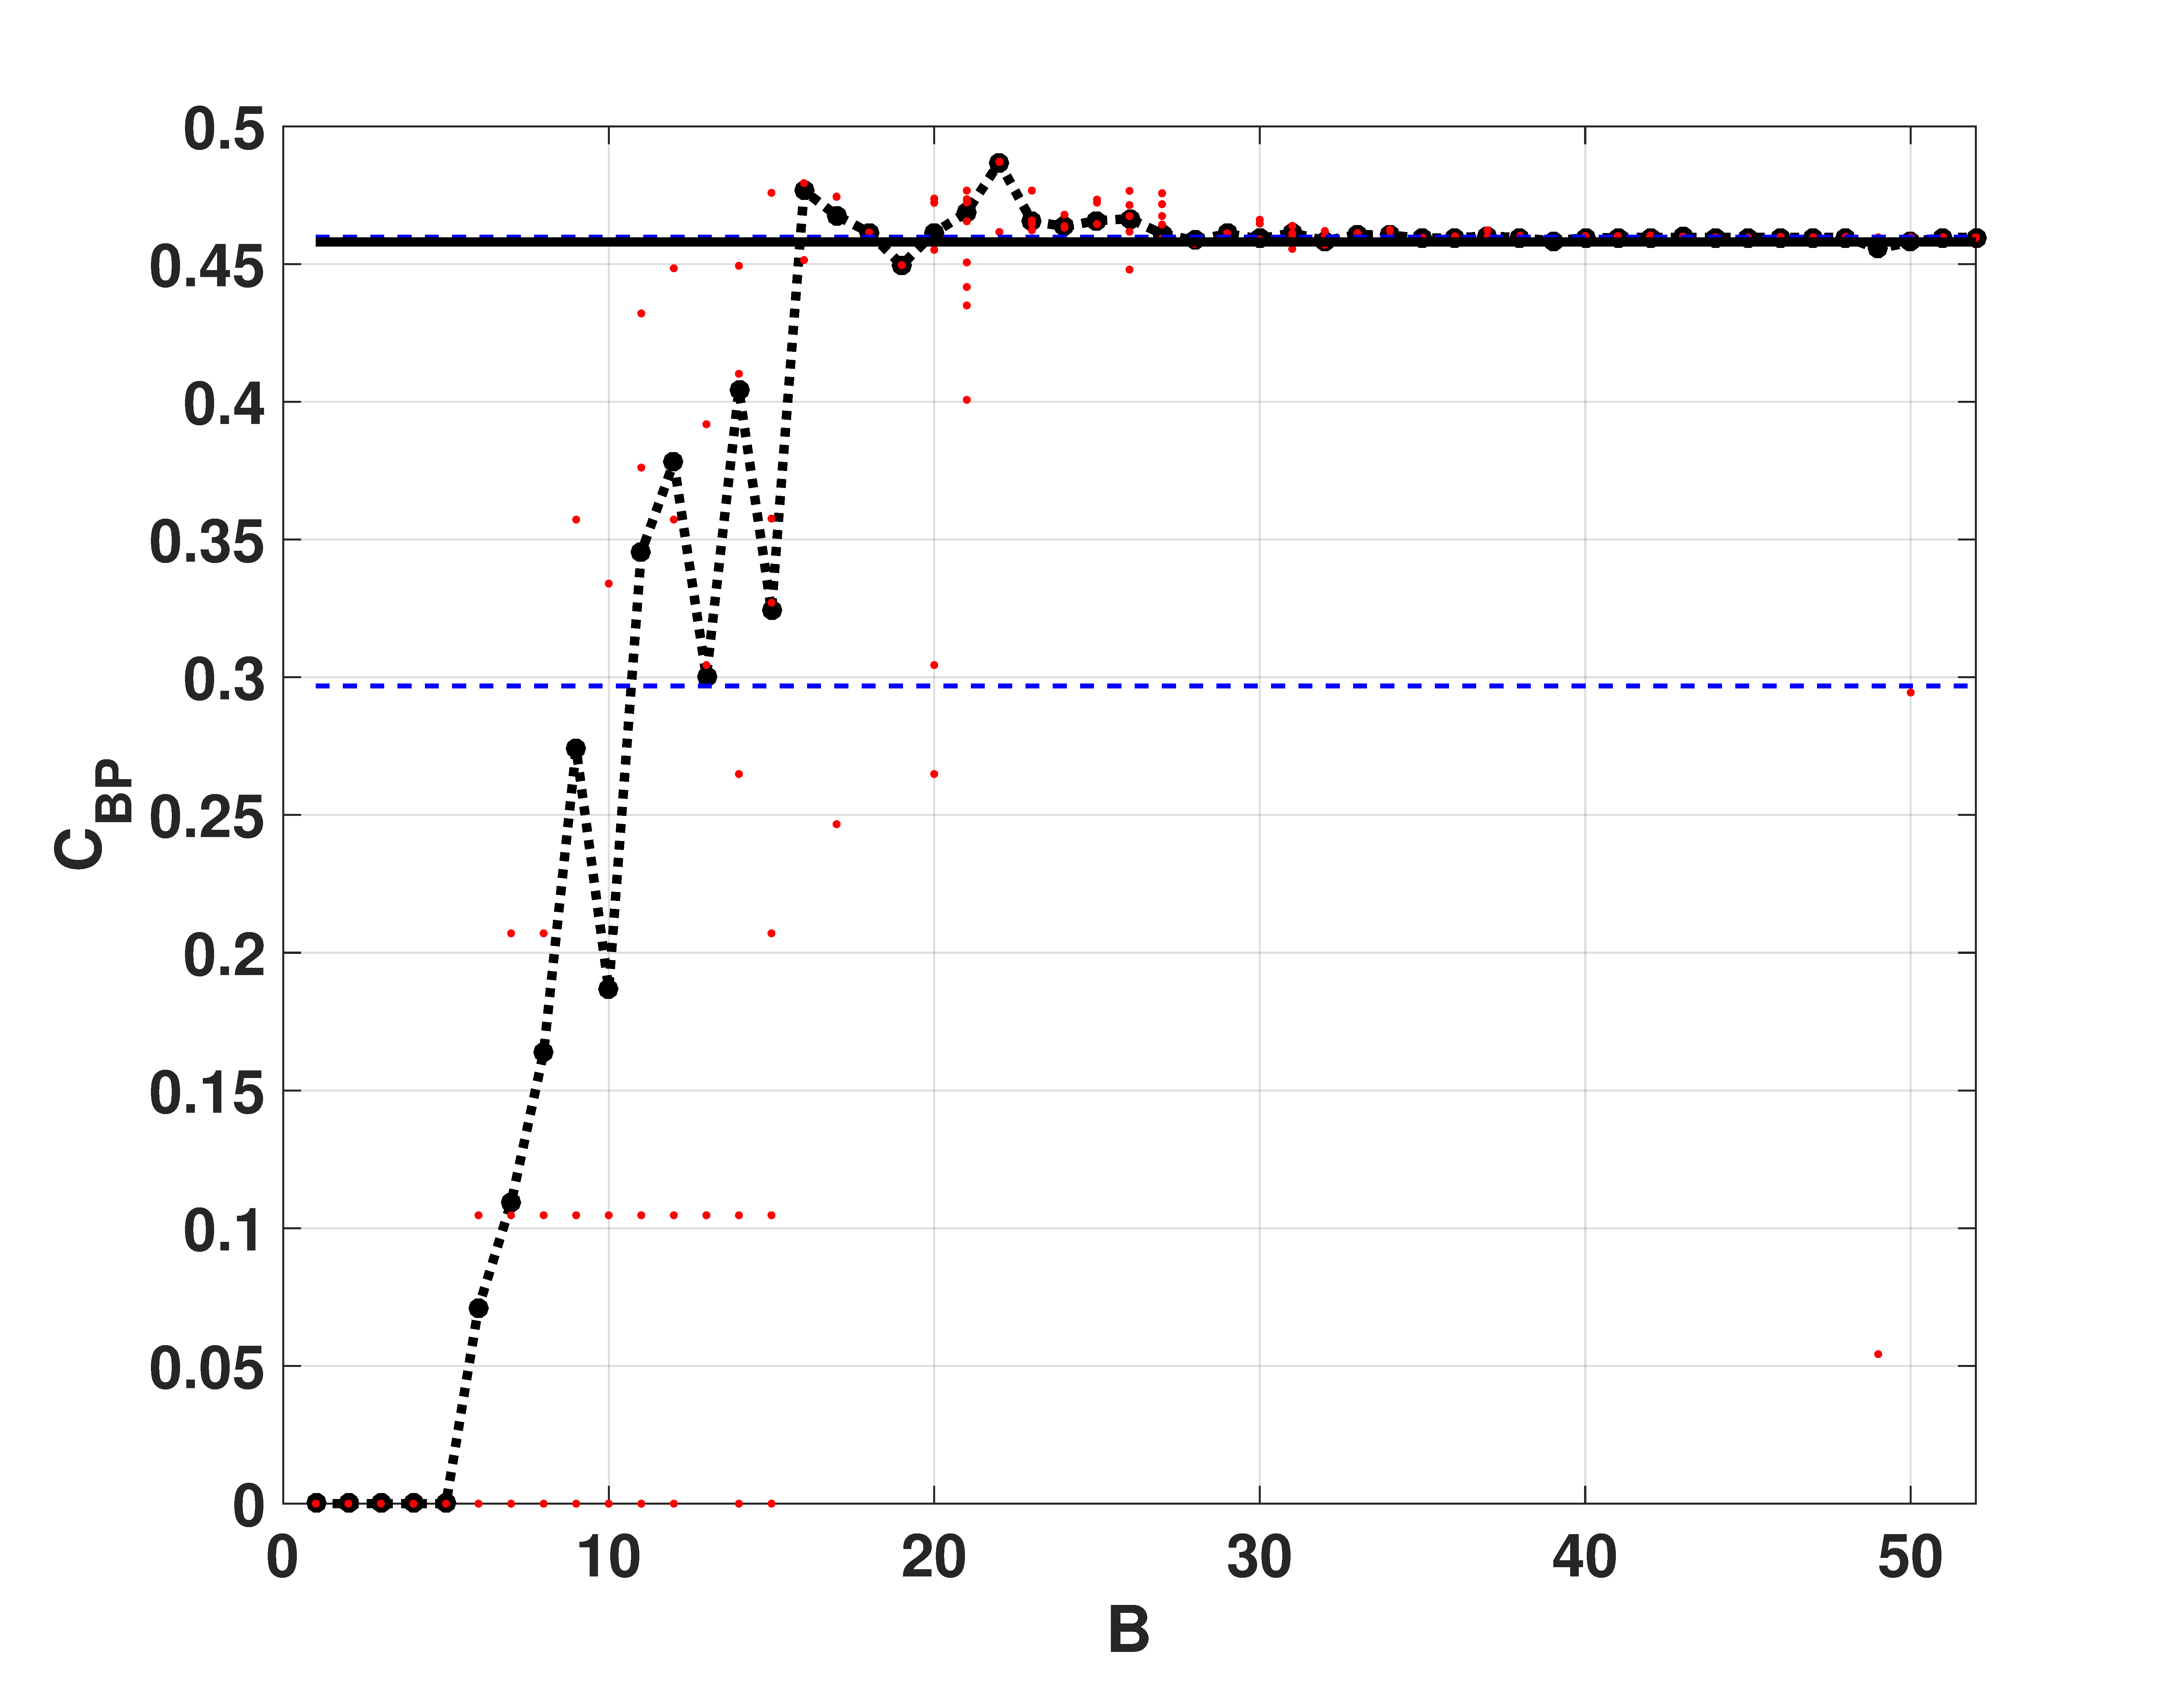
\includegraphics[width=\textwidth]{Cbp_Switch}
		\caption{$C_{BP}$ vs. $B$}
		\label{fig:Cbp_Switch}
	\end{subfigure}
	\begin{subfigure}[b]{0.49\textwidth}
		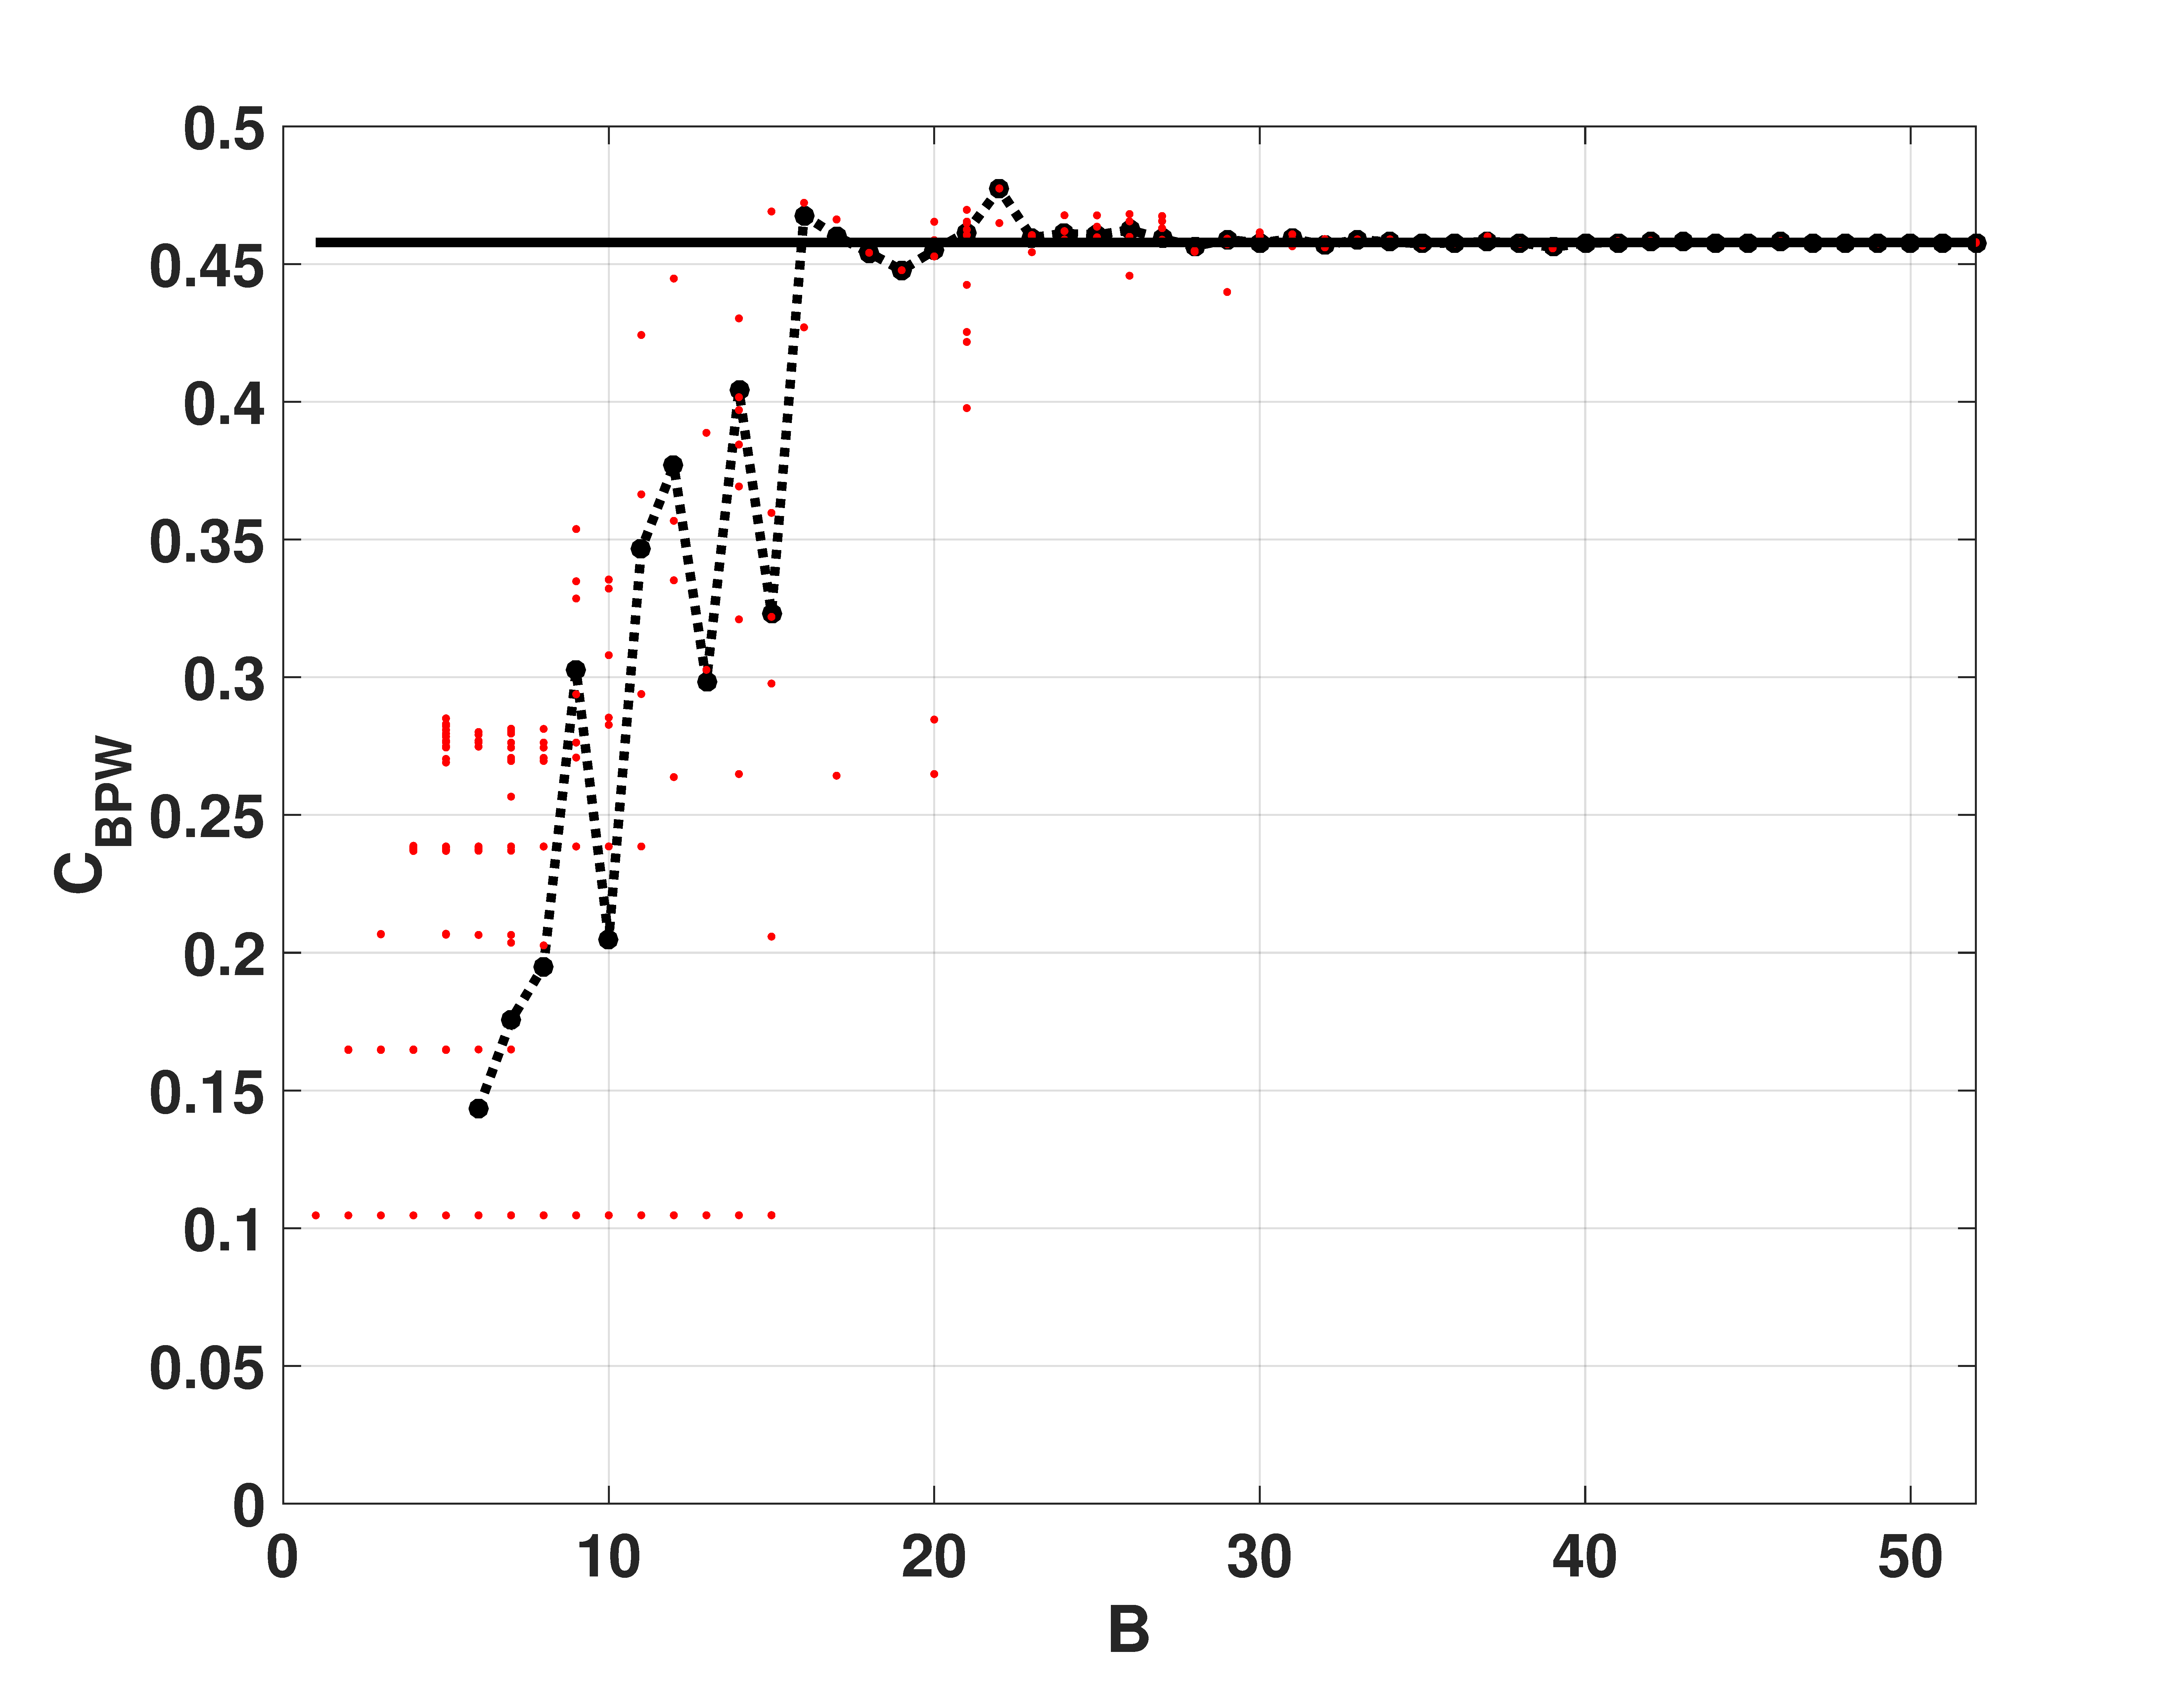
\includegraphics[width=\textwidth]{Cbpw_Switch}
		\caption{$C_{BPW}$ vs. $B$}
		\label{fig:Cbpw_Switch}
	\end{subfigure}
	\begin{subfigure}[b]{0.49\textwidth}
		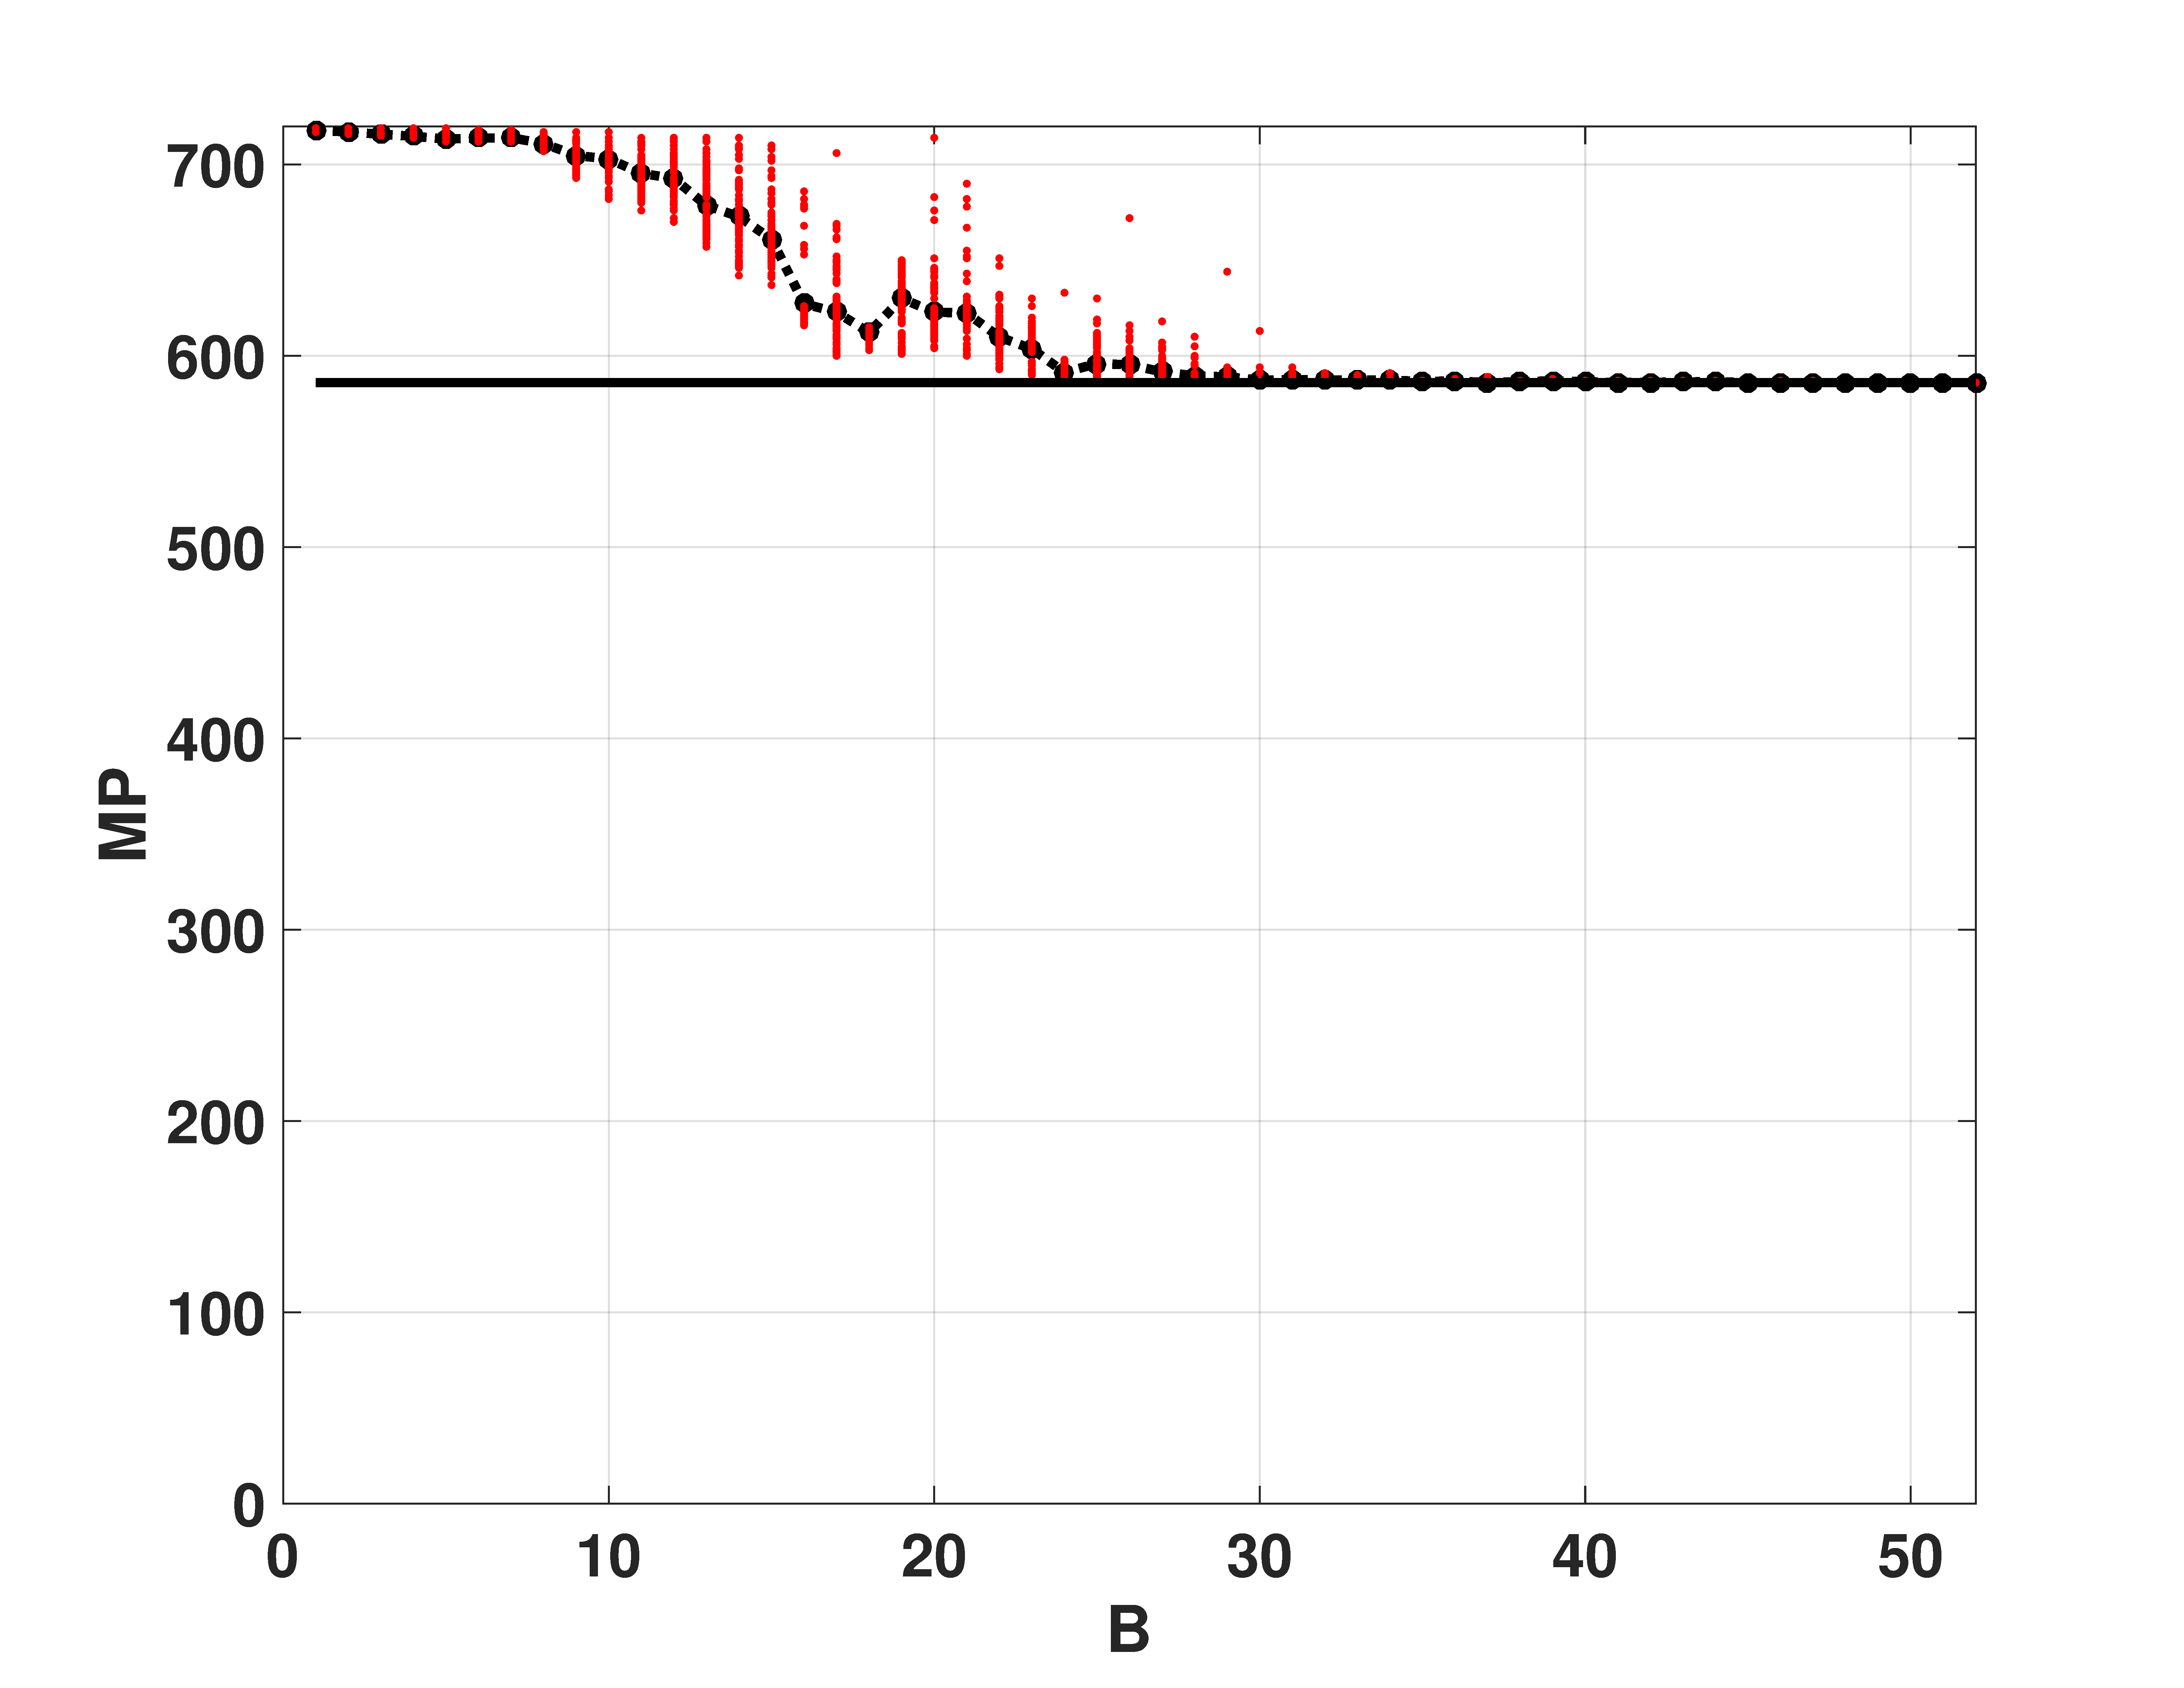
\includegraphics[width=\textwidth]{MP_Switch}
		\caption{MP vs. $B$}
		\label{fig:MP_Switch}
	\end{subfigure}
	\caption{Statistical properties of SWITCH map.}
	\label{fig:SWITCH_QuantiB}
\end{figure}

Double entropy plane $H_{hist} \times H_{BP}$ is showed in Fig. \ref{fig:SWITCH_HH}.
The reached point in this plane for SWITCH map is similar to that reached for LOG map, and it is denoted by a star in the figure.
The mixing is slight better in this case.

\begin{figure}[H]
	\centering
	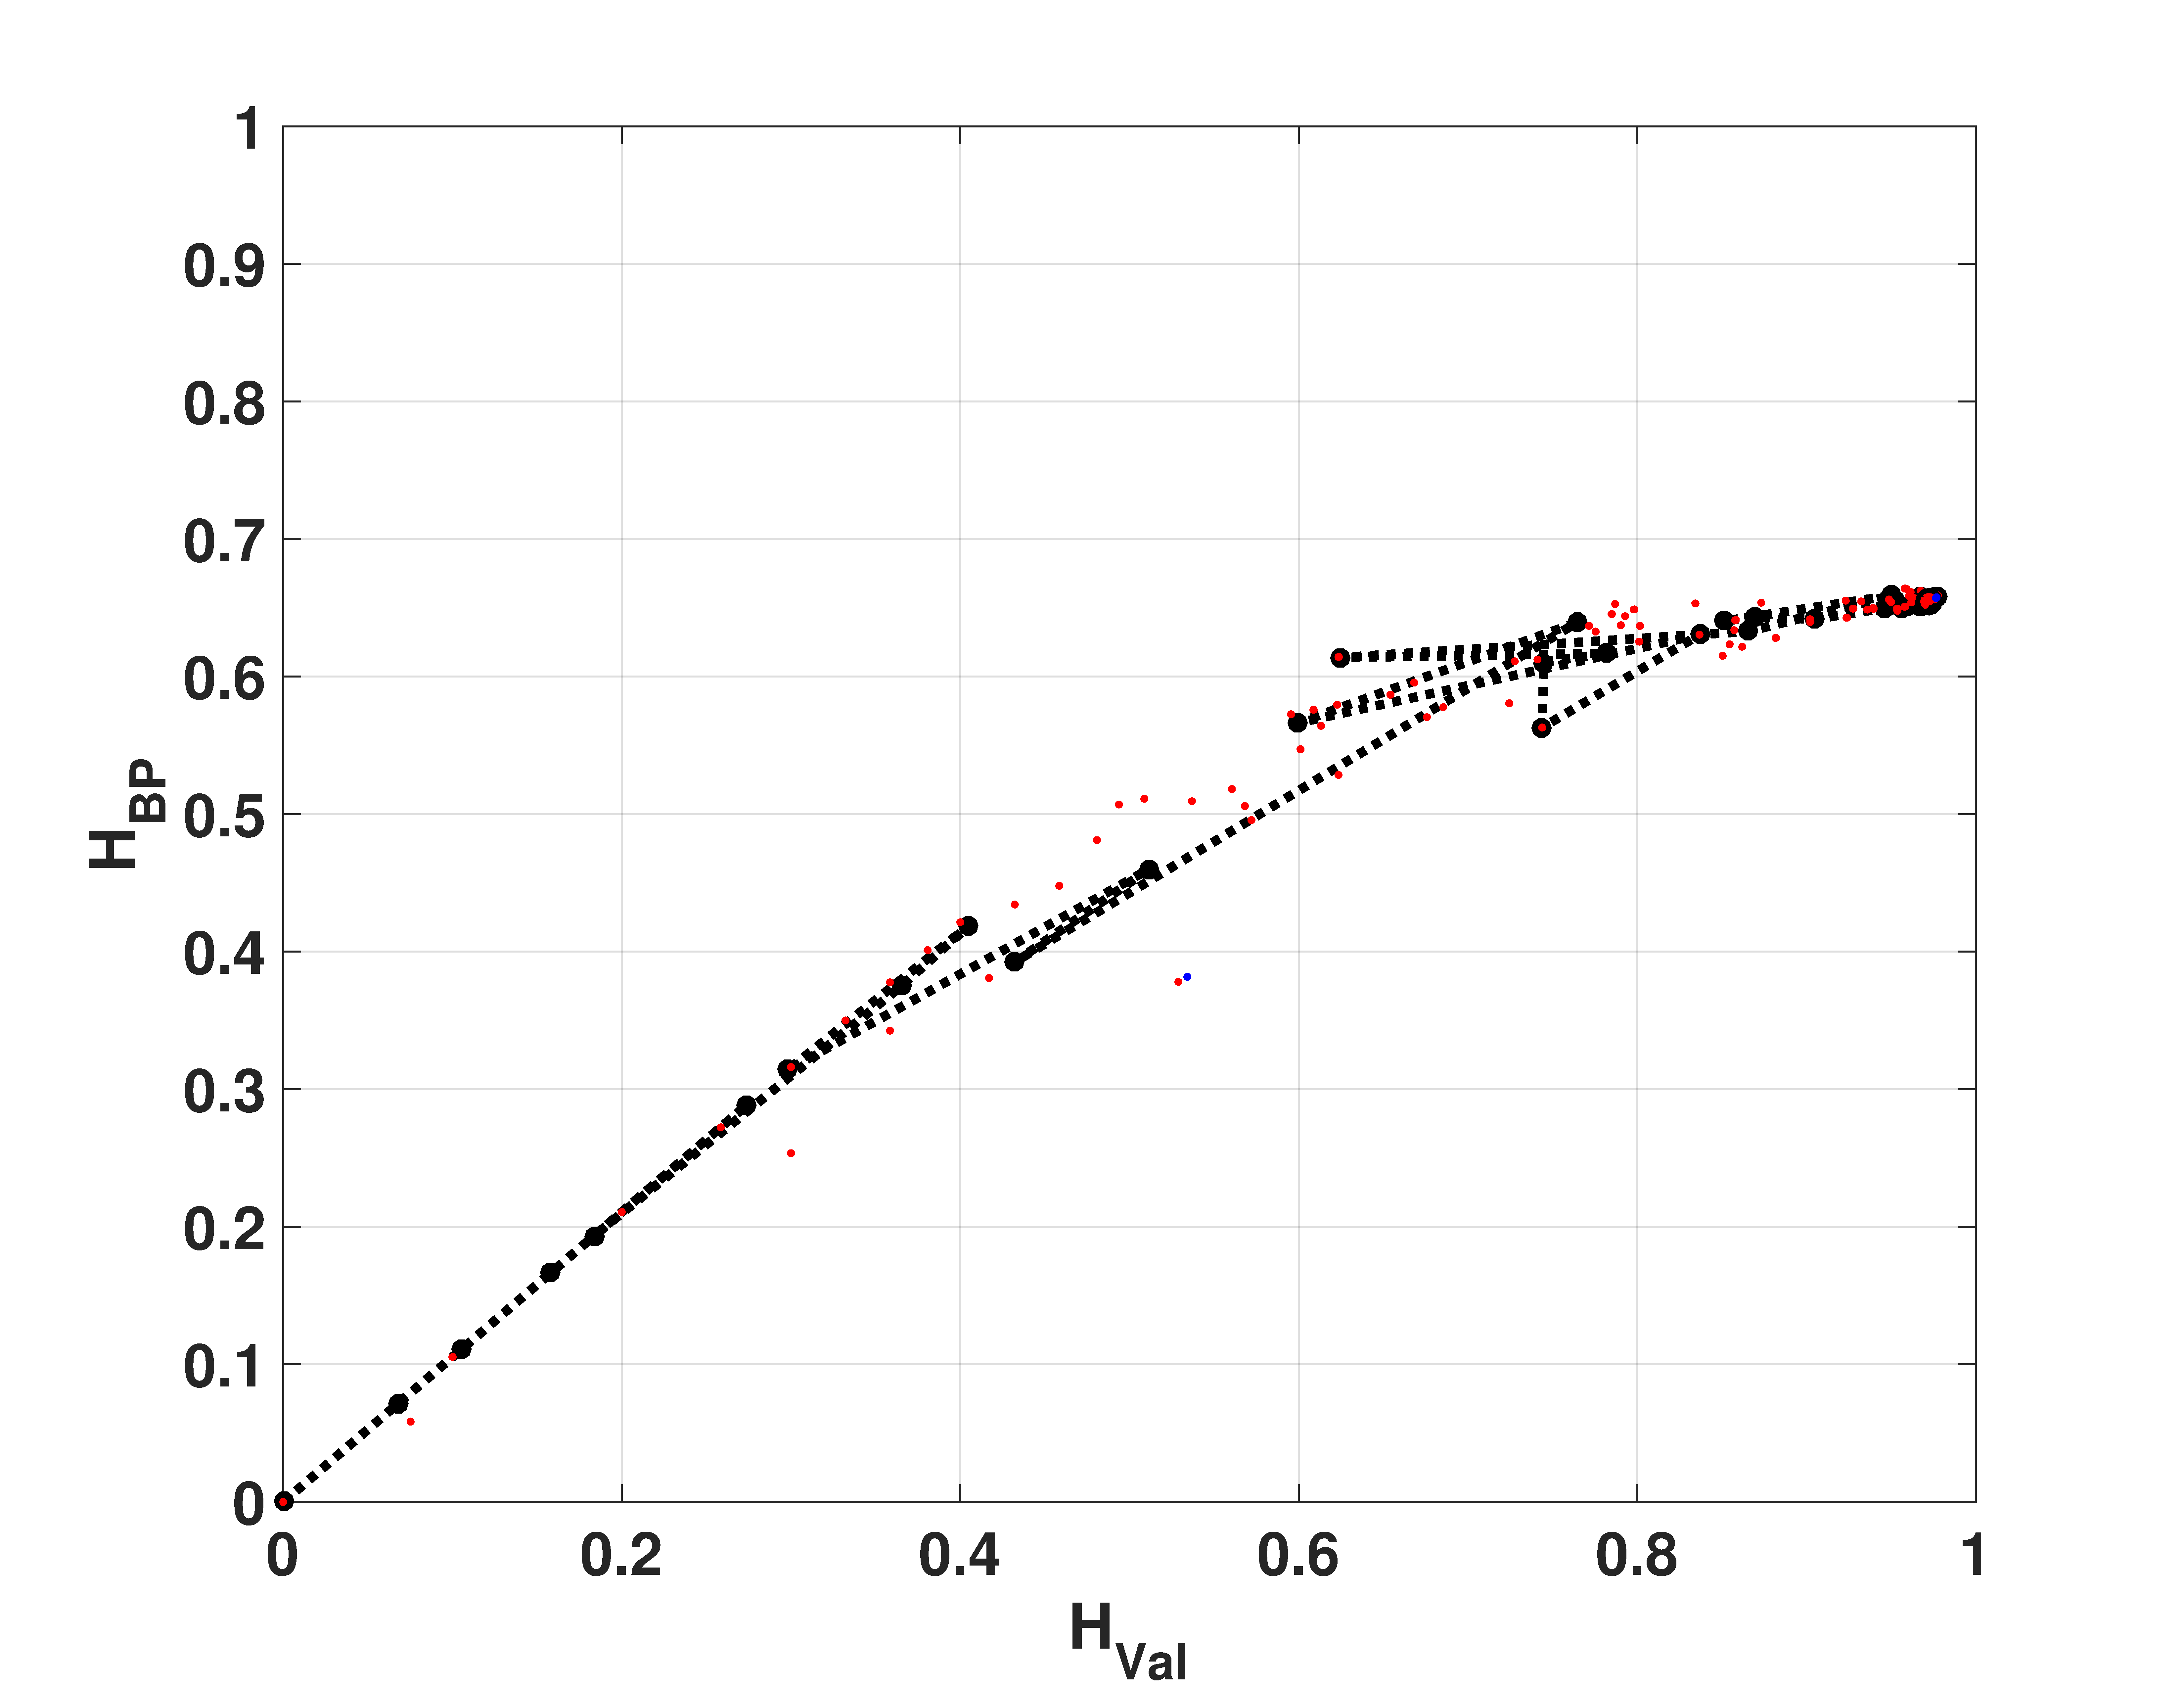
\includegraphics[width=.49\textwidth]{HbpHval_Switch}
	\caption{Evolution of statistical properties in double entropy plane for SWITCH map $H_{hist} \times H_{BP}$.}
	\label{fig:SWITCH_HH}
\end{figure}

Entropy-complexity plane $H_{BP} \times C_{BP}$ is showed in Fig. \ref{fig:SWITCH_HC}.
If we compare with the same plane in the case of LOG (Fig. \ref{fig:CbpHbp_Log}), $C_{BP}$ is lower for SWITCH, this fact shows a more random behavior.

\begin{figure}[H]
	\centering
	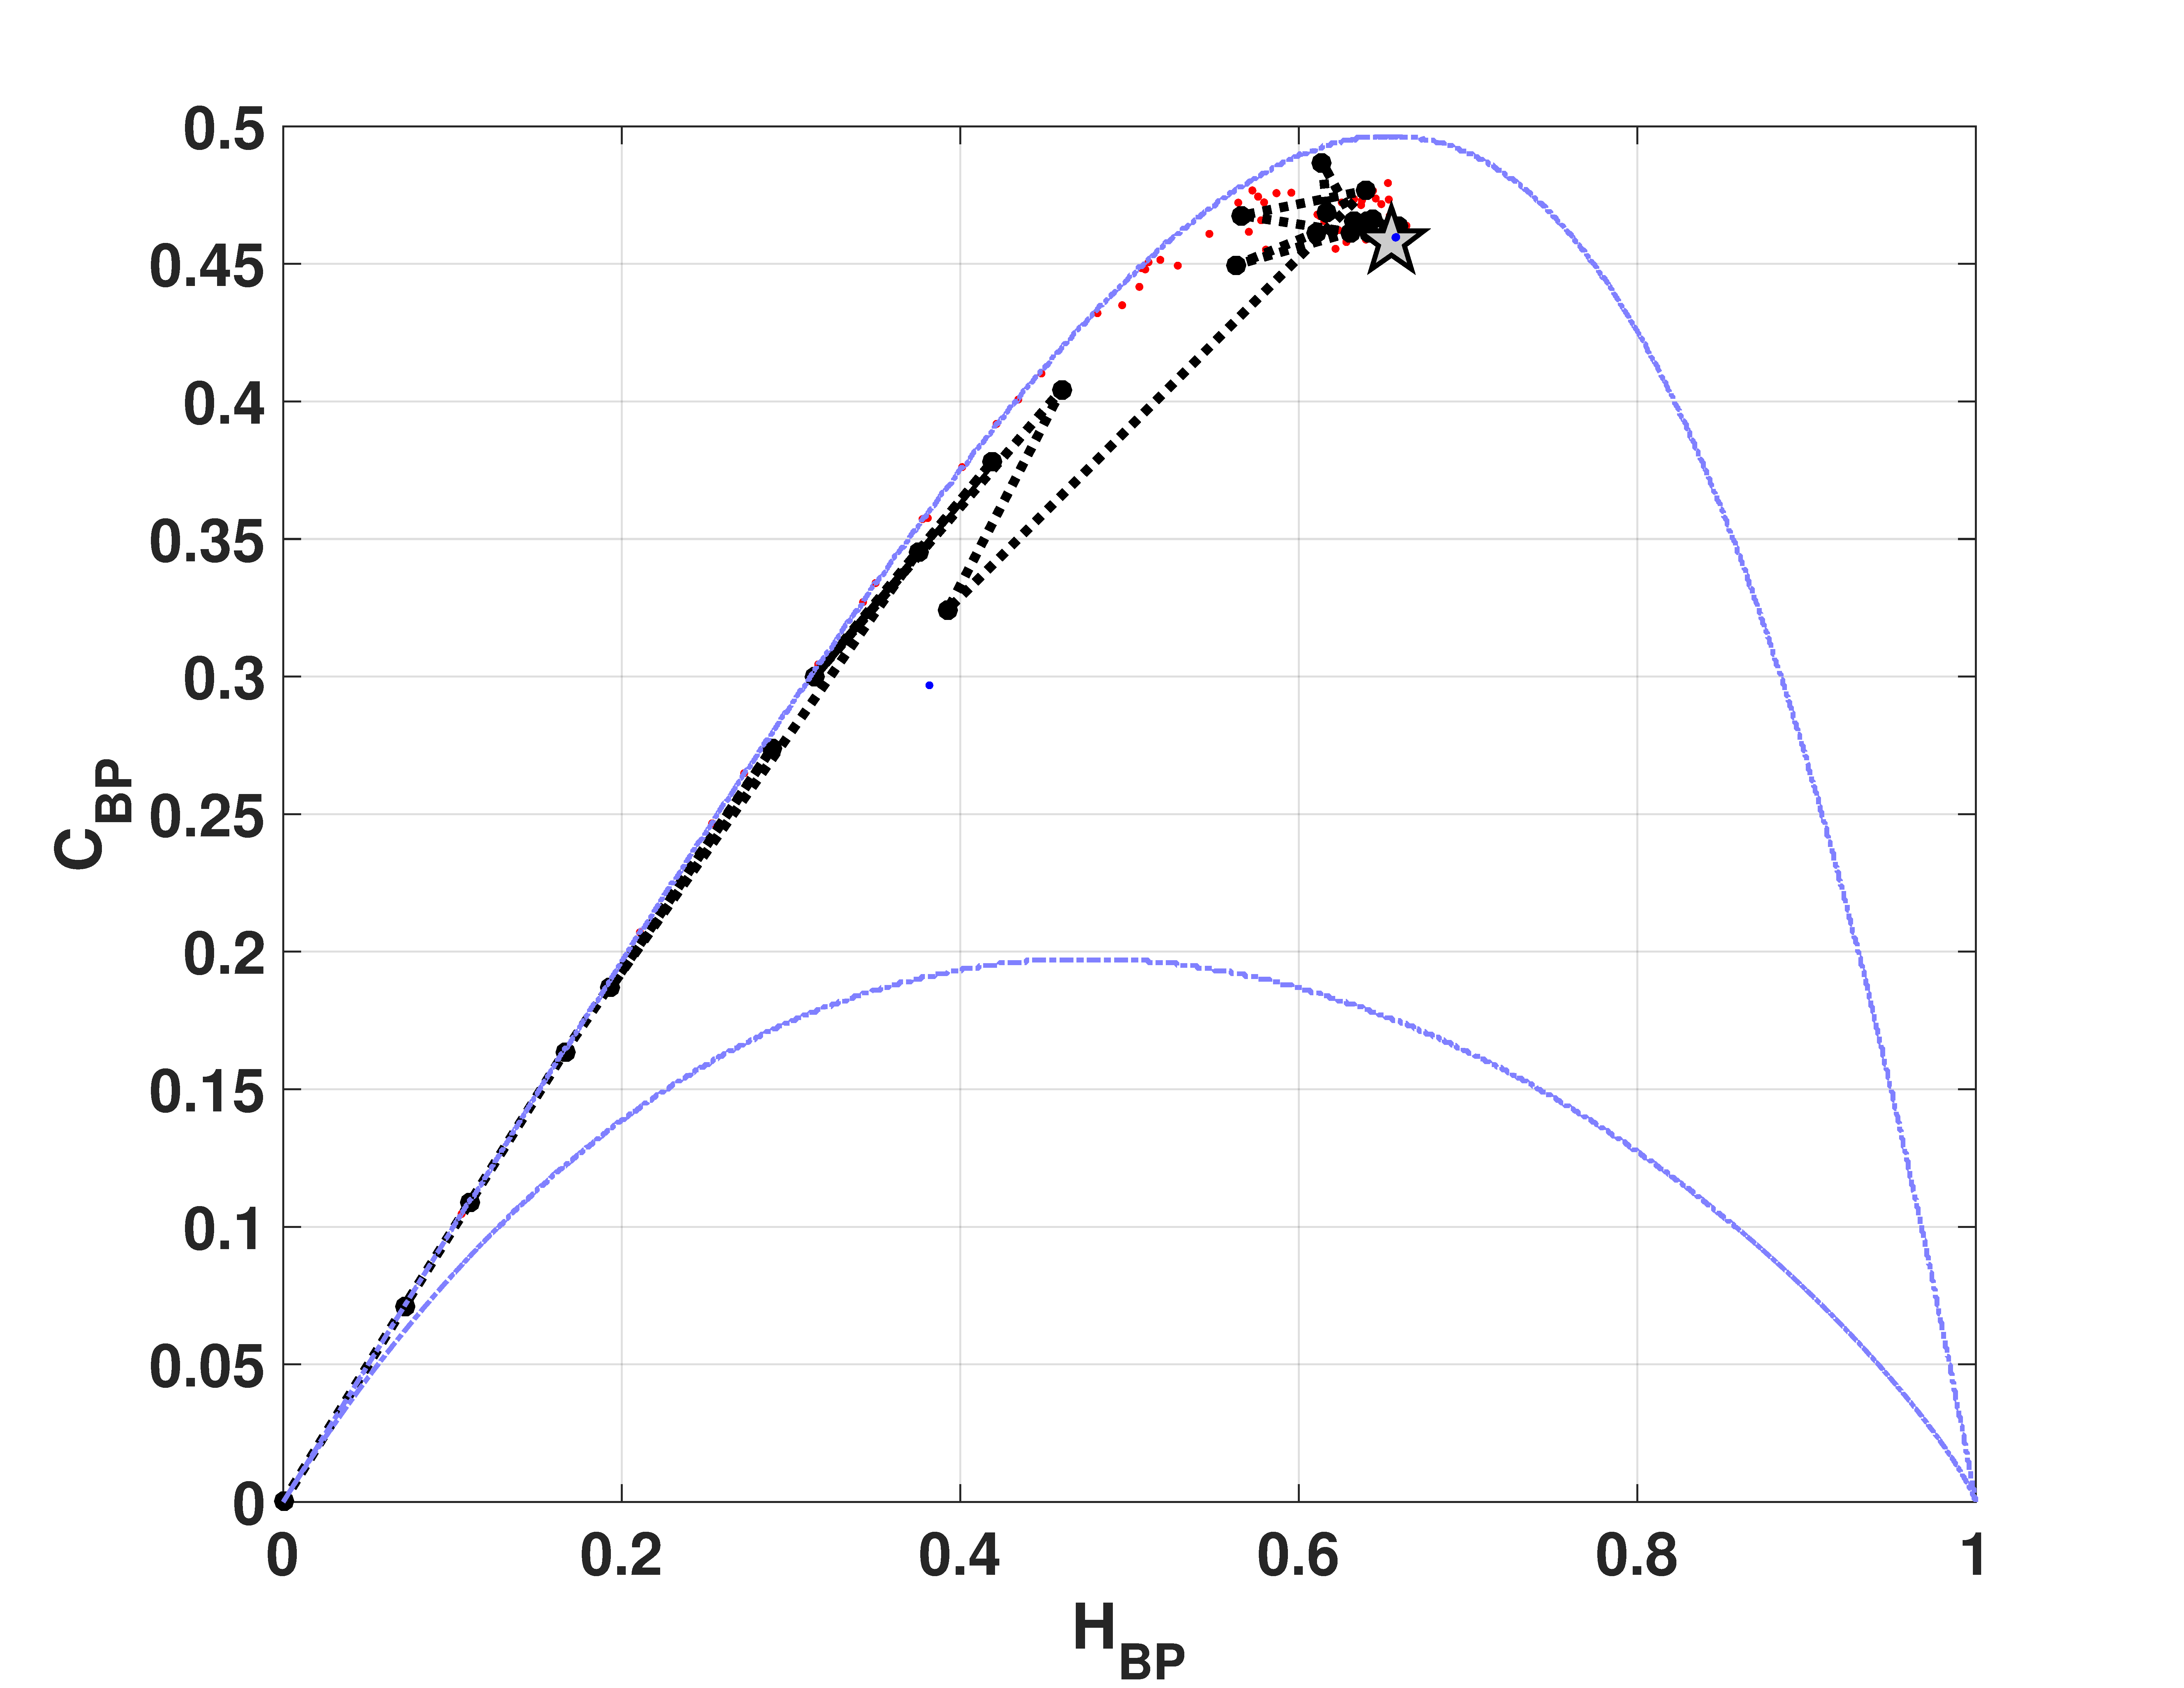
\includegraphics[width=.49\textwidth]{CbpHbp_Switch}
	\caption{Evolution of statistical properties in causal entropy-complexity plane for SWITCH map $H{BP} \times C_{BP}$.}
	\label{fig:SWITCH_HC}
\end{figure}